\chapter{Fundamentos teóricos y modelo matemático}

\par En este capítulo se presentan los conceptos teóricos, modelos matemáticos y algoritmos en el desarrollo del trabajo y realizar los cálculos que se describen luego en la sección de metodología.
\par En primer lugar se define un horno de proceso, se describe los tipos de hornos, sus componentes y las secciones generales que componen estos hornos. Por último, se presentan las ecuaciones necesarias para simular los fenómenos en cada sección del horno.

\section{Hornos de procesos}
\par Un horno de proceso es un intercambiador de calor de fuego directo que utiliza los gases calientes de la combustión para elevar la temperatura de una corriente que fluye a través de un serpentín de tubos alineados en todo el equipo.
\par Los hornos presentan distintas formas y configuraciones, dependiendo del fluido que se va a procesar en el equipo y el tipo de servicio que va a prestar; algunos hornos simplemente entregan el fluido de proceso a una temperatura predeterminada a la siguiente etapa del proceso de reacción; en otros se producen reacciones en el fluido mientras viaja a través de los tubos \cite{bib:biset}.

\subsection{Usos principales de los hornos}
\par Los hornos de proceso se utilizan en las industrias de procesamiento de hidrocarburos y productos químicos, como refinerías, plantas de gas, plantas petroquímicas, químicas y sintetizadoras de olefinas, amoníaco y fertilizantes. Algunas plantas pueden tener solo dos o tres calentadores, mientras que las plantas más grandes pueden tener más de cincuenta \cite{bib:thermox}.
\par La mayoría de las operaciones unitarias en estas plantas requieren uno o más hornos. Estas operaciones incluyen:
\begin{itemize}
    \item Alquilación.
    \item Coquización.
    \item Craqueo catalítico fluidizado.
    \item Craqueo térmico.
    \item Destilación.
    \item Hidrocraqueo.
    \item Reformado catalítico.
    \item Regeneración continua de catalizador.
\end{itemize}
Los hornos de proceso son utilizados como \cite{bib:thermox}:
\begin{itemize}
    \item Horno de arranque: pone en marcha una unidad de proceso donde se requiere calentar un lecho fluidizado de catalizador antes de agregar la carga.
    \item Horno rehervidor: proporciona calor a una columna de destilación calentando la parte inferior de la columna y vaporizando una parte de ella. Se usa cuando el requerimiento de calor es mayor que el que se puede obtener del vapor.
    \item Horno de craqueo: convierte moléculas más grandes en moléculas más pequeñas, generalmente con un catalizador (horno de pirólisis).
    \item Horno de calentamiento: lleva la corriente a la temperatura requerida para la siguiente etapa de reacción.
    \item Horno vaporizador: se utiliza para calentar y vaporizar parcialmente una carga antes de la destilación.
    \item Horno de petróleo crudo: calienta el petróleo crudo antes de la destilación.
    \item Horno reformador: usado en la conversión química del fluido mediante la adición de vapor y un catalizador contenido en los tubos.
    \item Horno de residuo: calienta el fluido a presiones menores a la atmosférica, normalmente el residuo de un flujo de petróleo crudo luego de un proceso de destilación.
    \item Horno de coquización retardada: calienta el flujo hasta la temperatura de coquización, para luego alimentar un tambor de coquización en línea.
\end{itemize}

\par Los hornos son definidos en función de su capacidad de suministro de calor ($Q_{absorbido}$) o carga, medida en MW o en millones de Btu/h. Para la mayoría de los hornos instalados en la industria petrolera, la capacidad suele oscilar entre 3 y 100 MW (10 y 350 MMBtu/h)\cite{bib:sandoval}.

\subsection{Secciones y componentes del horno}
\par En la Figura \ref{fig:horno} se presenta un horno de cabina, que se usa de modelo para describir sus secciones y componentes.

\subsubsection{Sección radiante}
\begin{figure} \begin{center}
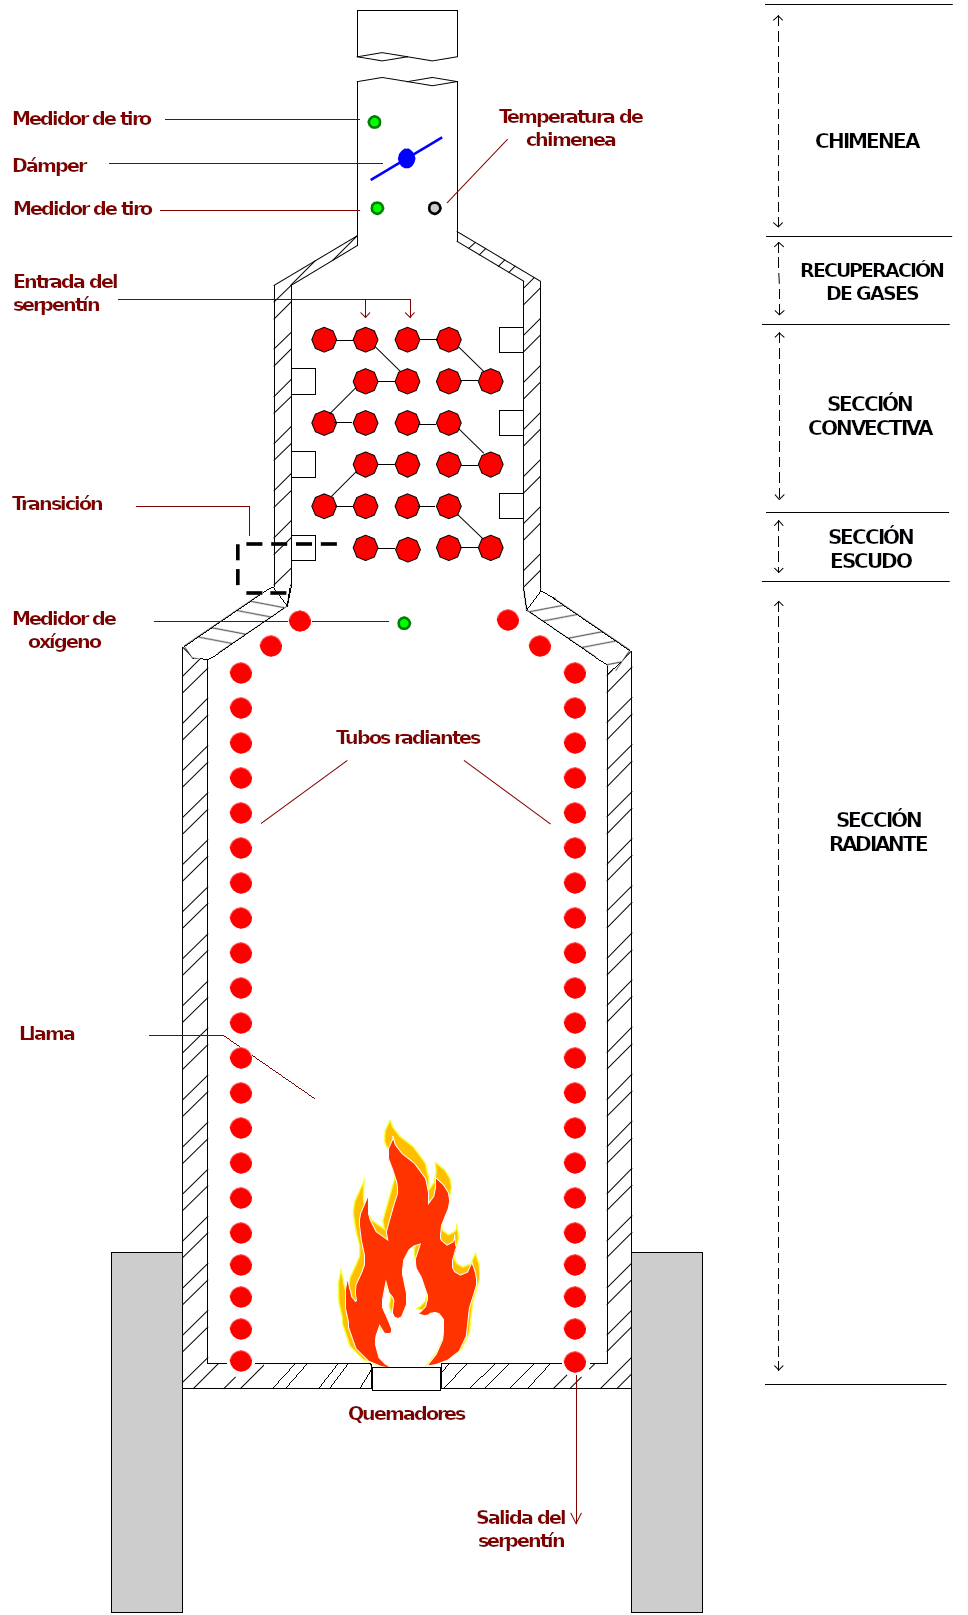
\includegraphics[scale=0.38]{images/horno}
\caption[Secciones de un horno]{Secciones de un horno de cabina.\cite{bib:thermox}}
\label{fig:horno} \end{center} \end{figure}
\par La zona radiante, o cámara de combustión, posee un revestimiento interno de material refractario, aquí se transfiere entre 60 y 70\% del calor requerido por el fluido.
\par En esta zona se ubica el haz de tubos lisos, por donde pasa el fluido, expuestos directamente a la radiación de la llama de combustión. Este puede ser de uno, dos, o mas pasos para la distribución del fluido.
\par También se encuentran los siguientes componentes:
\par \textbf{Carcasa}: son las paredes externas de acero del horno el cual encierra la sección de radiación del horno; por la alta temperatura de las paredes refractarias internas, en esta zona se pierde entre 1 y 5\% del calor de combustión al ambiente.
\par \textbf{Los quemadores}: es donde se realiza la mezcla de aire-combustible para luego atomizarlo y vaporizarlo para su posterior combustión. Se pueden ubicar en diferentes zonas de la sección de radiación, pueden ser de piso, techo, laterales o pared.
\par \textbf{Codos de retorno}: es la conexión de 180° de los tubos entre filas del serpentín. En esta área también se transfiere calor y se considera dentro del largo efectivo del tubo, a diferencia de la sección de escudo y convectiva.

\subsubsection{Transición (``crossover'')}
\par Comprende las tuberías que unen los serpentines de las secciones escudo y radiante. Están ubicadas fuera del horno y deben ser recubiertas con aislante de fibra refractaria y protegidas de la lluvia con láminas flexibles de aluminio.

\subsubsection{Sección de escudo}
\par Estos tubos están expuestos a radiación directa de la llama proveniente de la sección de radiación, y la transferencia de calor en esta zona a los tubos es aproximadamente 50\% por mecanismo de radiación y 50\% por convección. Suelen ser tubos del mismo diámetro que la sección de convección con la diferencia que estos siempre son lisos.
\par La medición del tiro debajo de esta sección (diferencias de presión entre la cámara de combustión y la atmósfera), es muy importante ya que determina la correcta configuración el horno. Este lugar también es ideal para medir el oxígeno de los gases de combustión y las partes por millón (ppm) de combustibles.

\subsubsection{Sección convectiva}
\par Los tubos de esta zona están fuera del alcance de la radiación de la llama de combustión y suelen presentar aletas. La transferencia de calor es en su mayoría por convección y los tubos se encuentran perpendiculares al flujo de gas.
\par Es la primera etapa de calentamiento del fluido de proceso y disminuyen, a su vez, la temperatura de los gases de combustión que salen del horno, aumentando el aprovechamiento de la energía y mejorando la eficiencia térmica.
\par También existen hornos sin área de convección, aunque éstos suelen tener una baja eficiencia y temperaturas de salida de los gases de combustión de alto riesgo operacional.

\subsubsection{Recuperación de gases de combustión}
El colector (“breeching” en ingles), existente principalmente en los hornos de hogar individual (cabina o cilíndrico) corresponde a la sección de transición entre el extremo rectangular de la sección convectiva con el extremo circular de la chimenea. Es un volumen vacío.

\subsubsection{Chimenea}
\par Es un conducto cilíndrico de acero, que permite la salida a la atmósfera de los gases de combustión del horno. Las chimeneas de los hornos modernos son revestidas con material refractario moldeable.

\subsubsection{Dámper}
\par La compuerta (Dámper), ubicada en el ducto de la chimenea, típicamente consiste de una placa plana conectada a un eje el cual puede ser rotado de manera similar a una válvula de mariposa. Actúa dando paso o reteniendo el flujo de los gases de combustión y regula de manera indirecta el flujo de aire que ingresa al horno y controla el tiro, o diferencia de presión, dentro del equipo.

\subsection{Clasificación de los hornos por diseño mecánico}
\par Los hornos son clasificados dependiendo de su diseño mecánico, como se puede apreciar en la Figura \ref{fig:hornos_tipos} las seis clasificaciones básicas son las siguientes \cite{pdvsa1}:
\begin{enumerate}[label=\Alph*]
    \item .-  Hornos tipo cilíndrico con serpentines verticales.
    \item .-  Hornos tipo cilíndrico con serpentín helicoidal.
    \item .-  Hornos tipo cabina doble con serpentines verticales.
    \item .-  Hornos tipo cabina con serpentín horizontal.
    \item .-  Hornos tipo cabina con serpentín pérgola.
    \item .-  Hornos de cabina doble con serpentines horizontales.
\end{enumerate}
\begin{figure}[hbt] \begin{center}
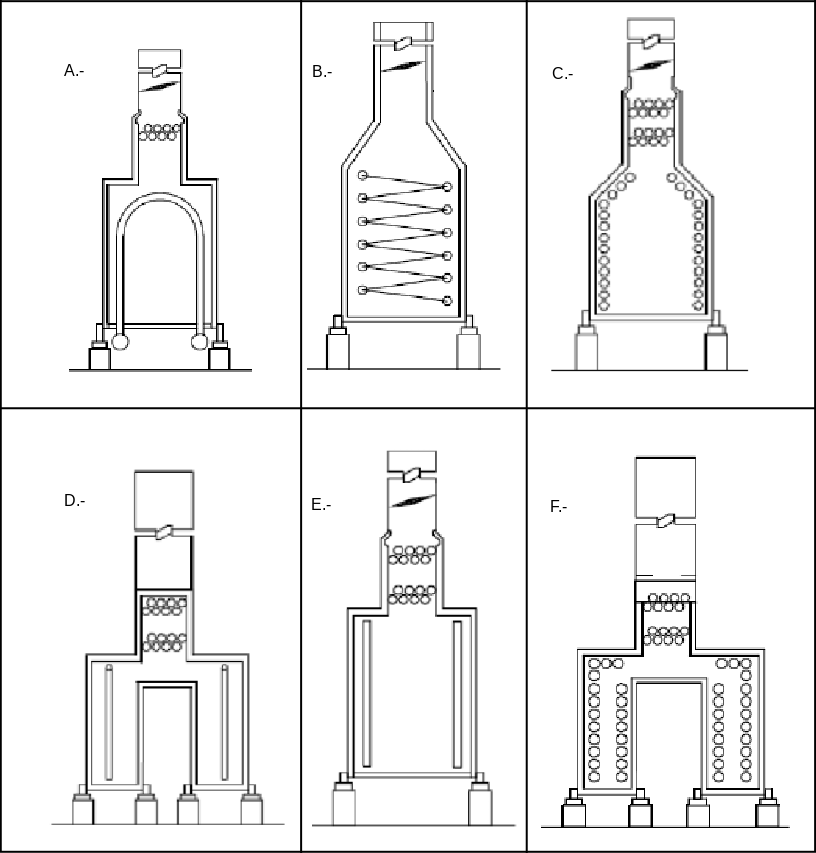
\includegraphics[scale=0.30]{images/hornos_tipos}
\caption[Tipos de hornos por diseño mecánico]{Clasificación de hornos según su diseño mecánico.\cite{kumar}}
\label{fig:hornos_tipos}
\end{center} \end{figure}

\subsection{Clasificación de los hornos por la ubicación de los quemadores}
\par Los quemadores se pueden instalar en el piso, las paredes o el techo de la sección radiante y la llama puede dirigirse hacia arriba, hacia los lados o hacia abajo. 
\par Los quemadores montados en la pared, con llama horizontalmente, pueden estar ubicados en la pared de fondo o en la pared lateral. Los quemadores de la pared de fondo producen llamas horizontales dirigidas a lo largo de la sección radiante. Los quemadores de pared lateral dirigen las llamas a lo ancho de la sección radiante \cite{kumar}. (ver Figura \ref{fig:quemadores})
\begin{figure}[H]
\begin{center}
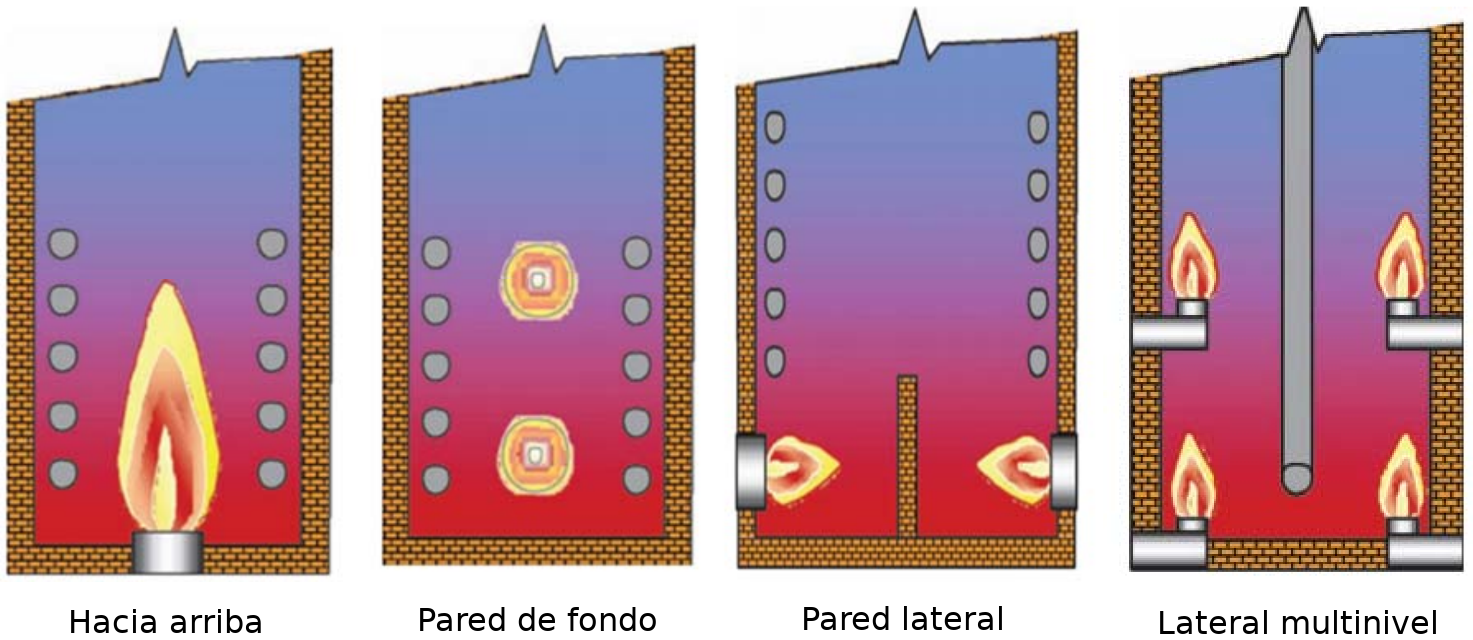
\includegraphics[scale=0.30]{images/quemadores}
\caption[Disposición de los quemadores]{Disposición de los quemadores.\cite{kumar}}
\label{fig:quemadores}
\end{center}
\end{figure}

\subsection{Clasificación de los hornos por el tiro (Draft)}
\par La diferencia entre la presión atmosférica y la presión del hogar (sección de radiación), se denomina tiro \cite{bib:draft}. El tiro es el resultado del flujo ascendente de los gases calientes dentro del horno debido a su menor densidad con respecto a densidad del aire atmosférico. Existen las siguientes clasificaciones de tiro para los distintos hornos.
\begin{enumerate}
    \item Tiro natural: es la configuración donde la columna caliente de gases en la chimenea y el horno provee la succión que atrae al aire para combustión al horno.
    \item Tiro forzado: en esta configuración se usa un ventilador para suplir el aire de combustión a los quemadores y para vencer la caída de presión a través de los quemadores.
    \item Tiro inducido: para esta configuración se usa un ventilador ubicado en la chimenea, que provee la succión adicional requerida (mayor que la suplida naturalmente), y mueve los gases de la combustión a través de la sección de convección.
    \item Tiro balanceado: es la combinación de las modalidades de tiro inducido y tiro forzado, teniendo un ventilador en la entrada del aire atmosférico y otro en la salida de los gases de combustión, como es el caso de los hornos equipados con precalentadores de aire.
\end{enumerate}

\section{Combustión de hidrocarburos}

\par El proceso de combustión consiste en la oxidación de los componentes del combustible y puede representarse mediante una ecuación química. Durante un proceso de combustión, la masa de cada elemento permanece igual. Por lo tanto, escribir ecuaciones químicas y resolver problemas relacionados con las cantidades de los distintos componentes implica básicamente la conservación de la masa de cada elemento. 
\par Cuando se quema un combustible de hidrocarburo, tanto el carbono como el hidrógeno se oxidan. Los productos de la combustión incluyen tanto dióxido de carbono como agua. El agua puede estar en fase vapor, líquida o sólida, dependiendo de la temperatura y presión de los productos de la combustión.
\par De la reacción química de combustión, del combustible seleccionado para el proceso, se libera el calor que luego es transferido al fluido dentro del horno.

\subsection{Combustión estequiométrica}
\par La combustión se da en la salida de los quemadores, espacio donde se mezcla el combustible con el oxígeno, normalmente extraído de una corriente de aire ambiental, cuya composición seca se aproxima en este proyecto a 20,95\% de oxígeno y 79,05\% de nitrógeno. Como ejemplo de esta reacción balanceada se puede observar la ecuación \ref{eq:combustion}, donde se usa metano como combustible, los moles de nitrógeno provienen de la relación volumétrica entre los compuestos del aire teórico seco 79,05/20,95 = 3,77.
\begin{equation}
    \label{eq:combustion}
    CH_4 + 2O_2 + 2(3,77)N_2 \rightarrow CO_2 + 2H_2O + 7,52N_2
\end{equation}
\par La mínima cantidad de aire que puede suministrar oxígeno suficiente para una reacción completa es llamado aire teórico. En la practica, la combustión completa no será lograda a menos que el aire suministrado sea mayor a 100\% del aire teórico, y cualquier valor superior es llamado exceso de aire.
\par Un parámetro importante, usualmente usado para expresar la relación de aire y combustible es la relación aire/combustible (designada como AC, ec. \ref{eq:ac}). Usualmente expresada en base másica, pero puedo encontrarse en base molar, como se muestra en la ecuación \ref{eq:ac}.
\begin{gather}
\label{eq:ac}
    AC_{masa} = \frac{m_{a}}{m_{c}}\\
    AC_{molar} = \frac{n_{a}}{n_{c}}
\end{gather}
\par Y se relacionan a través del peso molecular de la siguiente manera:
\begin{equation}
\label{eq:ac_rel}
    AC_{masa} = \frac{m_{a}}{m_{c}} =
    \frac{n_{a}*PM_{a}}{n_{c}*PM_{c}} = AC_{molar}*\frac{PM_{a}}{PM_{c}}
\end{equation}
\par Donde, $m$ es la masa, $PM$ el peso molecular, $n$ el número de moles y los subíndices $_a,_c$ corresponden al aire y el combustible respectivamente.

\subsection{Exceso de aire de combustión}
\par En un proceso de combustión real, la cantidad de aire se expresa como una fracción de la cantidad teórica. Una relación similar, denominada relación de equivalencia, es igual a la relación aire-combustible real dividida por la relación aire-combustible teórica, de la forma:
\begin{equation}
    \Phi = AC_{te\acute{o}rica}/AC
\end{equation}
\par Dado que el porcentaje teórico de aire y la relación de equivalencia vienen de la relación aire-combustible estequiométrica y la relación aire-combustible real, las masas moleculares se anulan y son las mismas ya sea que se utilice una base de masa o de mol.
\par Así, 150\% de aire teórico significa que el aire suministrado es 1,5 veces el aire teórico. La combustión completa de metano con 150\% de aire teórico, habiendo balanceado todos los coeficientes estequiométricos de conservación de todos los átomos, se escribe:
\begin{equation}
CH_4 + 1,5*2(O_2 + 3,77N_2 ) \rightarrow CO_2 + 2H_2O + O_2 + 11,28N_2
\end{equation}
\par Concepto que puede ampliarse para compuestos diferentes al metano y combinaciones de varios componentes, como es el gas de refinería.
\par La cantidad de aire realmente suministrada también puede expresarse en términos de porcentaje de exceso de aire. El exceso de aire es la cantidad de aire suministrada por encima del aire teórico. Así, 150\% de aire teórico equivale a 50\% de exceso de aire.

\subsection{Gases productos de la combustión}
\par Cuando la cantidad de aire suministrado es inferior al aire teórico requerido, la combustión es incompleta. Si sólo hay una ligera deficiencia de aire, el resultado habitual es que parte del carbono se une con el oxígeno para formar monóxido de carbono en lugar de dióxido de carbono. Si el aire suministrado es considerablemente menor que el aire teórico, también puede haber algunos hidrocarburos en los gases productos de la combustión.
\par Incluso cuando se suministra un exceso de aire, pueden estar presentes pequeñas cantidades de monóxido de carbono, dependiendo de una serie de factores físicos que incluyen la mezcla y la turbulencia durante la combustión. 
\par Otro factor a tomar en cuenta es la generación de óxidos de nitrógeno (NO$_x$) que se da debido a las altas temperaturas junto con la turbulencia encima de los quemadores de la sección de radiación. Se disocian las moléculas de oxígeno y el nitrógeno del aire se combina con los iones de oxígeno formando NO y NO$_2$.

\par Así, la combustión de metano con 10\% de exceso de aire podría ser como sigue \cite{bib:thermox}:
\begin{equation}
CH_4 + 1,1*2(O_2 + 3,77N_2) \rightarrow CO_2 + 2H_2O + ,2O_2 + 8,27N_2 + ppmCO + ppmH_2 + NO_X\end{equation}
\par Incrementar el exceso de aire reduce la temperatura de la llama y disminuye la eficiencia térmica del horno. Cuanto más exceso de aire, más oxígeno hay disponible para producir NO$_x$. Por el contrario, cuanto menos oxígeno, menos posibilidades de formación de NOx y aumento en la formación de CO (ver Fig. \ref{fig:nox}).
\begin{figure}[H] \begin{center}
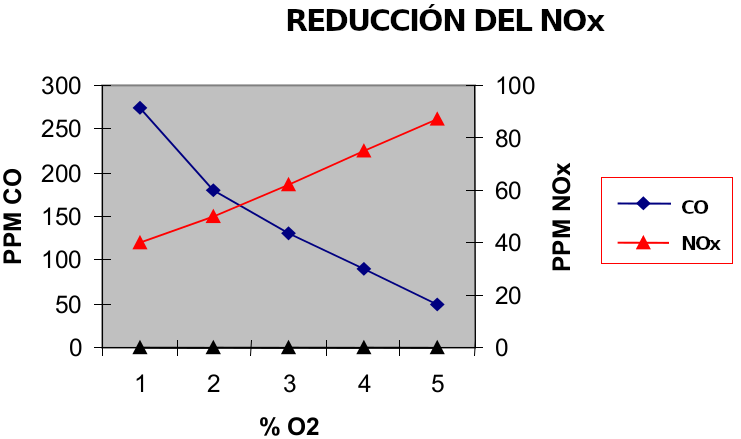
\includegraphics[scale=0.42]{images/nox}
\caption[Reducción del NO$_x$ al disminuir el exceso de aire de combustión]{Reducción del NO$_x$ al disminuir el exceso de aire.\cite{bib:thermox}}
\label{fig:nox} \end{center} \end{figure}
\par De las emisiones de NOx producidas anualmente, 16\% se puede atribuir a la industria química/refinación, y los estrictos límites de emisión requieren un mayor control del NOx y otros componentes de la chimenea. Operar el horno con una eficiencia óptima, con bajo exceso de aire, es la forma más sencilla y menos costosa de reducir las emisiones de NOx \cite{bib:thermox}.

\subsection{Exceso de oxígeno en los gases de combustión}
\par Un análisis de los productos de la combustión proporciona un método muy simple para calcular la cantidad real de aire suministrado en un proceso de combustión. Existen varios métodos experimentales mediante los cuales se puede realizar dicho análisis. Algunos arrojan resultados en base seca y otros procedimientos experimentales dan resultados que incluyen el vapor de agua. 
\par El principio básico al utilizar el análisis de los productos de la combustión para obtener la relación aire-combustible real es la conservación de la masa de cada elemento. Por lo tanto, al cambiar de reactivos a productos, podemos hacer un balance de carbono, un balance de hidrógeno, un balance de oxígeno y un balance de nitrógeno (además de cualquier otro elemento que pueda estar involucrado).
\par Dentro de la combustión estequiométrica completa que se usa en el simulador, el exceso de aire puede obtenerse al definir un exceso de oxígeno y viceversa. 

\subsection{Humedad del aire}
\par El aire utilizado en la combustión es aire húmedo ambiental, por lo tanto el agua del aire debe ser considerada en los cálculos de combustión.
\par El valor normalmente usado para referirse a la humedad del aire es la humedad relativa, $HR$, y es la relación entre la presión de vapor actual, $p_w$ y la presión de saturación:
\begin{equation}
    HR = 100 * p_w/p_s
\end{equation}
\par Para el cálculo de la presión parcial de saturación del vapor de agua en el aire se usa la ecuación de Tetens \cite{bib:tetens} descrita a continuación:
\begin{equation}
    p_s = 610,78 * e^{t/(t +238,3)*17,2694}
\end{equation}
\par Donde $t$ es la temperatura del aire en grados celcios, que puede ser corregida para temperas de congelación ( $<$ 0 ºC) como se muestra en la ecuación \ref{eq:ice}.
\begin{equation}
\label{eq:ice}
    p_{s-hielo} = -4,86 + 0,855p_s + 0,000244p_s^2
\end{equation}
\par De esta manera, usando como datos de entrada la humedad relativa y la temperatura del aire se conoce la presión parcial del vapor de agua en el aire y por tanto su contenido de agua para ser usado en los cálculos de combustión del horno.

\subsection{Entalpía y energía interna de combustión}
\par La entalpía de combustión, h$_{RP}$, se define como la diferencia entre la entalpía de los productos y la entalpía de los reactivos con combustión completa evaluada a una temperatura y presión dadas. Eso es,
\begin{equation}
\begin{gathered}
\bar h_{RP} = H_P - H_R \\
\bar h_{RP} = \sum_P n_e(\bar h^0_f + \Delta \bar h)_e - \sum_R n_i(\bar h^0_f + \Delta \bar h)_i
\end{gathered}
\end{equation}
\par La entalpía de combustión es habitualmente expresar por unidad de masa de combustible, kilogramo $(h_{RP})$ o kilomol $(\bar h_{RP})$ de combustible.
\par Como la entalpía de formación es fija, podemos separar los términos como:
\begin{equation}
    H = H^0 + \Delta H
\end{equation}
\par Dónde
\begin{equation}
    H^0_{R} = \sum_R n_i \bar h^0_{fi} ; \quad \Delta H_{R} = \sum_R n_i \Delta \bar h_{i}
\end{equation}
\par Y
\begin{equation}
    H^0_{P} = \sum_P n_i \bar h^0_{fi} ; \quad \Delta H_{P} = \sum_P n_i \Delta \bar h_{i}
\end{equation}
\par Ahora la diferencia de entalpías se escribe
\begin{equation}
\begin{gathered}
    H_P - H_R = H^0_P - H^0_R + \Delta H_P - \Delta H_R \\
    \quad \quad = H^0_{RP} + \Delta H_P - \Delta H_R
\end{gathered}
\end{equation}

\par Mostrando explícitamente la entalpía de combustión de referencia, $H^0_{RP}$, y los dos términos de partida $\Delta H_{P}$ y $\Delta H_{R}$. Los últimos dos términos para los productos y reactivos son distintos de cero si existen en un estado distinto al estado de referencia.
\par Los valores de entalpía para la combustión requieren una temperatura y presión de referencia, la entalpía de formación usada tiene una de 25°C y 0,1 MPa, esta fue obtenida de las tablas de entalpía de Borgnakke y Sonntag \cite{bib:vanwylen}.
\par La energía interna de combustión se define de manera similar.
\begin{equation}
\begin{gathered}
    U_{RP} = U_{P} - U_{R} \quad\quad\quad\quad\quad
    \quad\quad\quad\quad\quad\quad\quad\quad\quad\quad\quad\quad\quad\quad\\
    = \sum_P n_e (\bar h^0_{f} + \Delta \bar h - P\bar v)_{e} - \sum_R n_i (\bar h^0_{f} + \Delta \bar h - P\bar v)_{e}
\end{gathered}
\end{equation}
\par Cuando todos los componentes gaseosos se pueden considerar como gases ideales, y el volumen de los componentes líquidos y sólidos es insignificante en comparación con el valor de los componentes gaseosos, esta relación para $\bar u_{RP}$ se reduce a
\begin{equation}
        U_{RP} = H_{RP} - \bar RT (n_{productos gaseosos} - n_{reactivos gaseosos})
\end{equation}

\subsection{Poder calorífico}
\par El poder calorífico, o calor de reacción, representa el calor transferido desde una cámara durante la combustión o reacción a temperatura constante. En el caso de un proceso de presión constante, o de flujo constante, se deduce de la ecuación de la energía que es igual al negativo de la entalpía de combustión. Por esta razón, esta transferencia de calor a veces se denomina poder calorífico a presión constante para los procesos de combustión.
\par Cuando se usa el término poder calorífico (CV, de sus siglas en inglés), se usan los términos poder calorífico superior e inferior (groso y neto). El poder calorífico superior (``gross calorific value'', GCV) es la transferencia de calor con agua líquida en los productos, y el poder calorífico inferior (``net calorific value'', NCV) es la transferencia de calor con agua vaporizada en los productos.
\par La ecuación del energía para un flujo constante es ahora escrita como:
\begin{gather}
\label{eq:cv}
\begin{gathered}
U_{RP} = H_R - H_P \quad\quad\quad\quad\quad\quad\\
0 = \bar H^0_{RP} + \Delta H_R - \Delta H_P
\end{gathered}\\
 NCV = \Delta H_{P_{vapor.de.agua}} - \Delta H_R \quad
\end{gather}
\par Si los reactivos y los productos entran y salen en las condiciones de referencia, la energía neta que sale es igual al poder calorífico. Para situaciones en las que los reactivos se precalientan, $\Delta H_R > 0$, la salida de energía neta es correspondientemente mayor, y si los productos salen a una temperatura elevada, $\Delta H_P > 0$, que es lo típico, la salida de energía neta se reduce. Se deben evaluar todos los términos con la misma escala que la base de masa o mol.

\subsection{Temperatura de llama adiabática}
\par Es la temperatura máxima de los productos de la combustión. La temperatura de llama adiabática, en un flujo constante de productos, se encuentra a partir de la ecuación \ref{eq:llama} de energía, quedando como:
\begin{equation} \label{eq:llama}
\begin{gathered}
    H_R = H_P \\
    \sum_R n_i (\bar h^0_{f} + \Delta \bar h)_{i} = \sum_P n_e (\bar h^0_{f} + \Delta \bar h)_{e}
\end{gathered}
\end{equation}
\par Entonces, para un proceso de combustión sin trabajo ni transferencia de calor, los dos primeros términos definen la entalpía del producto, y la temperatura del producto se denomina temperatura de llama adiabática. La temperatura depende del estado de los reactivos y de la composición de los productos, por lo que la temperatura de llama adiabática máxima ocurre si los reactivos se suministran a la temperatura de referencia ($\Delta H_R$ = 0) y la combustión es completa, de modo que el se conoce la composición del producto \cite{bib:vanwylen}.
\par Para un combustible dado y una presión y temperatura dadas de los reactivos, la temperatura de llama adiabática máxima que se puede lograr es con una mezcla estequiométrica. La temperatura de la llama adiabática se ve afectada por la cantidad de exceso de aire que se utiliza.

\section{Balances de energía en el horno}
\par Con los aspectos anteriormente definidos se puede plantear un balance de energía global, usando el horno como volumen de control, Ec. \ref{eq:balance-global}, donde se aprecia la distribución del calor generado en la combustión. Ver la Figura \ref{fig:balance-energic}.

\begin{figure}[hbt]
\begin{center}
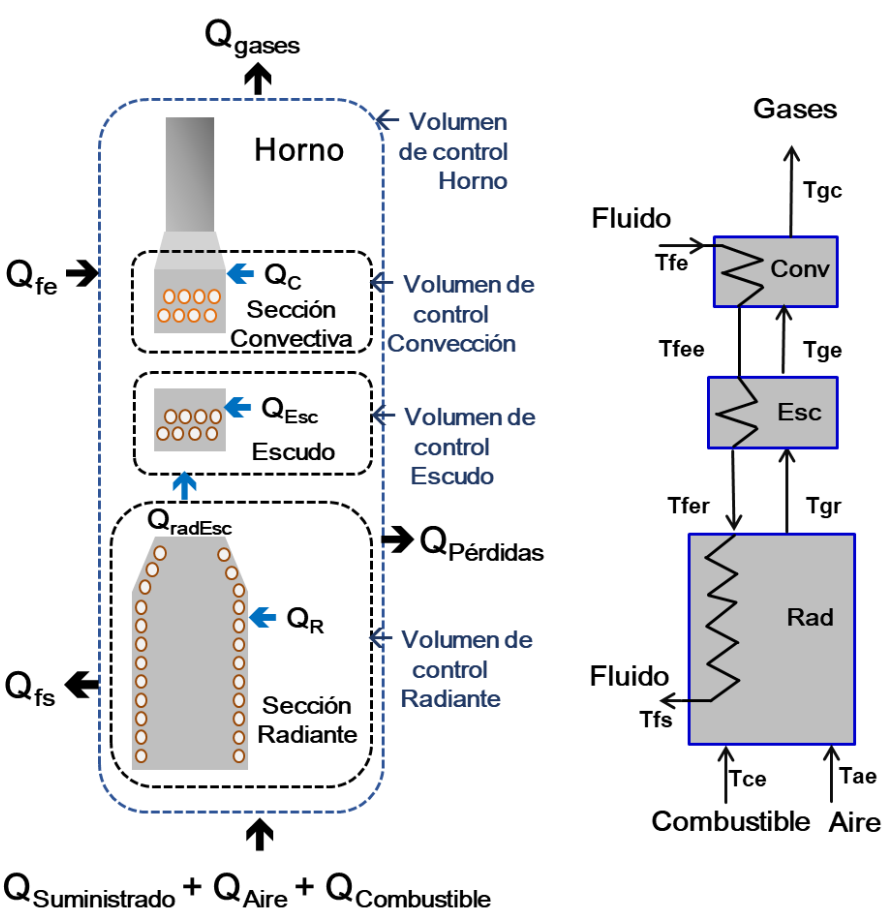
\includegraphics[scale=0.38]{images/balance-energic}
\caption[Balance de energía del horno]{Balance global de energía en el horno y similitud con intercambiador de tres etapas.}
\label{fig:balance-energic}
\end{center}
\end{figure}

\begin{equation}
    \label{eq:balance-global}
    \begin{gathered}
    Q_{entrada} = Q_{salida}\\
    Q_{suministrado} + Q_{a} + Q_{c} = 
    Q_{g} + Q_{f} + Q_{perdidas}
    \end{gathered}
\end{equation}
\par Donde:\\
$Q_{suministrado} = NCV * \dot m_{c}$\\
$Q_{a} = \dot m_{a} * Cp_{a}(T) * (T_{a_e} - T_{ref})$\\
$Q_{c} = \dot m_{c} * Cp_{c}(T) * (T_{c_e} - T_{ref})$\\
$Q_{g} = \dot m_{g} * Cp_{g}(T) * (T_{g_c} - T_{ref})$\\
$Q_{f} = \dot m_{f} * Cp_{f}(T) * (T_{f_s} - T_{f_e})$\\
$Q_{perdidas} =$ Pérdidas de calor al ambiente por las paredes del horno.
\par Como se pudo apreciar en la descripción de tipos de horno, el arreglo mecánico puede variar pero para fines de este análisis las tres zonas o volúmenes de control son: radiante, escudo y convectiva. 
\par El volumen de control radiante corresponde a la sección de radiación del horno, donde está presente la llama de la combustión.
\par La división de la sección superior del horno se debe a que dos zonas presentan diferencias en los mecanismos de transferencia de calor; así, los tubos de la zona escudo reciben radiación luminosa directa de la llama, que no está presente en la zona convectiva.
\par La zona de escudo en este análisis está formada por las dos primeras filas de tubos y son tubos lisos, mientras que la zona convectiva está conformada generalmente por tubos con aletas. En ambas zonas está presenta la radiación del gas y la reflectada de las paredes de la sección hacia los tubos. Esta radiación, de baja longitud de onda, deja de ser significativa por debajo de los 550 °C (1022 °F).
\par Conociendo que la energía transferida al fluido de proceso es igual a:
\begin{equation}
    \begin{gathered}
    Q_{fs} - Q_{fe} = Q_{RAD} + Q_{ESC} + Q_{CONV}\\
    \quad\quad\quad\quad = \dot m_f * C_{p_f} * (T_{fs} - T_{fe})
    \end{gathered}
\end{equation}
\par Donde $Q_{RAD}, Q_{ESC}, Q_{CONV}$ son el calor que transfieren los gases de combustión al fluido en las zonas radiante, de escudo y convectiva respectivamente y que corresponde al servicio del horno, substituyendo en ecuación \ref{eq:balance-global}.
\begin{equation}
    Q_{suministrado} + Q_{a} + Q_{c} = Q_{RAD} + Q_{ESC} + Q_{CONV} + Q_{perdidas} + Q_{g}
\end{equation}
\par Para cuantificar el balance del honor es necesario cuantificar los calores $Q_{RAD}$, $Q_{ESC}$, $Q_{CONV}$ y de esta forma:
\begin{enumerate}
    \item Calcular la cantidad de combustible requerido por el servicio, $Q_{suministrado}$.
    \item Calcular el comportamiento del horno ante variaciones de las condiciones operacionales, tales como, cambios en: la composición de combustible, el exceso de aire, la cantidad de fluido que circula, el requerimiento de temperatura de salida del fluido, los factures de ensuciamiento, etc.
\end{enumerate}

\subsection{Zona Radiante}
\par En la zona radiante, los tubos que transportan el fluido de proceso reciben radiación directa desde la llama del quemador y las paredes refractarias. En esta zona la transmisión de calor entre los gases de combustión y el banco de tubos se estima en 85\% por radiación, y 15\% por convección.
\par El análisis descrito a continuación está basado en el modelo presentado inicialmente por Lobo \& Evans \cite{bib:rad} y parte de la suposición de un mezclado ideal de los gases producto de la combustión en la sección radiante; lo cual implica una temperatura uniforme del gas en todo el volumen de la sección radiante, denominada temperatura de arco radiante $T_g$, la que será la temperatura efectiva de transferencia de calor entre los gases de combustión y la superficie de los tubos, y será igualmente la temperatura de entrada de los gases de combustión hacia el escudo de tubos, $T_{gr}$.
\par Realizando el balance de energía en el volumen de control de la sección radiante resulta:
\begin{equation}
    \label{eq:rad}
    Q_{suministrado} + Q_{a} + Q_{c} = 
    Q_{RAD} + Q_{radEsc} + Q_{CONV} + Q_{perdidas} + Q_{g}
\end{equation}
\par En la zona radiante se transfiere calor al fluido por dos mecanismos, mediante radiación directa y por convección entre los gases producto de la combustión y el fluido:
\begin{equation}
    \label{eq:rad-fluid}
    Q_{RAD} = Q_{rad} + Q_{conv} = \dot m_f * C_{p_f} * (T_{fs} - T_{fer})
\end{equation}
\par Donde $Q_{rad}, Q_{conv}$ son el calor que se transfiere al fluido en la sección radiante por radiación y por convección, y $Q_{radEsc}$ es el calor por radiación que se transfiere a los tubos de la zona escudo desde la zona radiante.
\par Usando las ecuaciones de transferencia de calor, modificadas para la radiación en hornos \cite{bib:mekler}, y de convección:
\begin{gather}
\label{eq:radiac}
    Q_{rad} = \sigma *(\alpha *Acp)_{RAD} *F *(T_{g}^{4} -T_{w}^{4})\\
    Q_{radEsc} = \sigma *(\alpha *Acp)_{ESC} *F *(T_{g}^{4} -T_{w}^{4})\\
    Q_{conv} = h_{c} * A_t * (T_g - T_w)
\end{gather}
$\sigma$ = Constante de Stefan-Boltzmann (W/m$^2$-K$^4$).\\
$\alpha$ = Factor de efectividad relativa del banco de tubos.\\
$Acp$ = Área del plano frontal a la llama del banco de tubos (m$^2$).\\
$A_t$ = Área total externa del banco de tubos (m$^2$).\\
$F$ = Factor de transferencia radiante.\\
$T_g$ = Temperatura efectiva del gas en la zona radiante (K).\\
$T_w$ = Temperatura promedio de la pared del tubo (K).\\
$h_c$ = Coeficiente convectivo de la zona radiante (W/m$^2$°C).
\par Se estima que las pérdidas de calor por las paredes del horno son una fracción, $F_p$, entre 1 y 5\%, del calor suministrado, quedan los calores definidos:
\begin{equation}
    Q_{perdidas} = F_p * NCV * \dot m_c
\end{equation}
\par Y de la masa del combustible y la relación aire-combustible se obtiene la masa de los gases de combustión:
\begin{equation}
    \dot m_g = \dot m_c * AC_{masa} + \dot m_c = \dot m_c (1 + AC_{masa})
\end{equation}
\par Substituyendo en las ecuaciones (\ref{eq:rad}) y (\ref{eq:rad-fluid}) se obtiene:
\begin{equation}\label{eq:rad-tgr}
\begin{gathered}
\dot m_c*NCV + \dot m_a*C_{p_a} * (T_a -T_{ref}) 
+ \dot m_c*C_{p_c} * (T_c -T_{ref}) = \\
\dot m_c*(1 +AC_{masa}) * C_{p_g} * (T_g -T_{ref}) + \\
\sigma *(\alpha *Acp)_{RAD}*F*(T_g^4-T_w^4) + 
\sigma *(\alpha *Acp)_{ESC}*F*(T_g^4-T_w^4) + \\
h_{c}*A_t*(T_g -T_w) + 0,015*\dot m_c*NCV
\end{gathered}
\end{equation}
\begin{equation}
\begin{gathered}
\label{eq:rad-comp}
Q_R = 
\sigma * (\alpha *Acp)_{RAD} *F *(T_g^4 -T_w^4) +h_{c} *A_t *(T_g -T_w)\\
= \dot m_f * C_{p_f} * (T_{fs} - T_{fer})
\end{gathered}
\end{equation}
\par La ecuación (\ref{eq:rad-comp}) permite calcular la  temperatura efectiva de llama $T_{g}$, usando el método numérico de Newton Rapshon, descrito en el Apéndice \ref{apx:met}, a partir de un estimado del calor transferido al fluido en la zona radiante ($Q_{RAD} = 70\% Q_{absorbido}$). Y finalmente, la ecuación (\ref{eq:rad-tgr}) permite calcular el flujo másico de combustible requerido, $\dot m_C$, de forma directa.

\subsubsection{Temperatura promedio de pared de tubos ($T_w$)}
\par La temperatura promedio de pared de los tubos de la zona radiante es calculada a partir de la ecuación de transferencia de calor entre el fluido y la pared externa del tubo:
\begin{equation}
    q_{rad} = Q_R / A_o
\end{equation}
\par Donde $q_{rad}$ es el flujo de calor por unidad de área exterior del tubo (densidad de flujo de calor) en la zona radiante.
\begin{gather*}
q_{rad} = \frac{(Q_{rad} + Q_{conv})}{A_o} = (T_w - T_b) / (A_t *\Sigma R) \\
\Sigma R = R_{int} + R_{fi} + R_{tubo}
\end{gather*}
\par Que corresponden a la resistencia convectiva interna, el factor de ensuciamiento y la resistencia conductiva de la pared del tubo. Resolviendo por $T_w$
\begin{equation}
\label{eq:tw}
T_w = q_{rad} *(d_o/d_i) *[ R_{fi} + 1/h_i + d_i*ln(d_o/d_i)/(2k_f) ] +T_b
\end{equation}

\par Donde,\\
$T_b$ es la temperatura de mezcla del fluido $(T_{fs} + T_{fer})/2$. \\
$k_f$ es la conductividad térmica del tubo. \\
$h_i$ es el coeficiente interno de transferencia de calor. \\
$R_{fi}$ es el factor de ensuciamiento interno del tubo. \\

\par Para resolver la ecuación (\ref{eq:tw}) se necesita calcular la temperatura de entrada del fluido a la zona radiante, $T_{fer}$ a partir del estimado de $Q_{RAD}$. 

\subsubsection{Coeficiente interno de transferencia de calor (coeficiente de película del fluido)}
\par El coeficiente interno de transferencia de calor es calculado para líquidos por la ecuación modificada de Colburn:
\begin{equation}
\label{eq:hi}
 h_i = 0,023 * \frac{k_f}{d_i} *Re^{0,8} *Pr^{1/3} *(\mu_b /\mu_w )^{0,14}
\end{equation}
\par Donde,\\
$\mu_b$ y $\mu_w$, son las viscosidades del fluido de proceso a $T_b$ y $T_w$. \\
G, es el flujo másico por unidad de área. \\
Re = $(\rho v d_i / \mu)_b = (G *d_i / \mu)_b$. Número de Reynolds evaluado a $T_b$.\\
Pr = $(\mu C_p / k)_f$. Número de Prandtl del fluido de proceso evaluado a $T_b$.

\subsubsection{Coeficiente convectivo de la zona radiante}
\par El coeficiente convectivo de la parte exterior de los tubos en la zona radiante, para un horno tipo cabina con tubos en la pared donde no existe un patrón de flujo definido, se ha estimado en \cite{sirios}:
\begin{equation}
h_{c} = 1,5 BTU/hr.ft^2.^{\circ}F \approx 8,5 W/m^2.^{\circ}C)
\end{equation}

\subsubsection{Área de plano frontal que reemplaza el área de los tubos $(Acp)_{RAD}$}
\par Las superficies normales de absorción de calor en un horno consisten en una serie de tubos paralelos. En el caso de un diseño de hornos donde los tubos se reciben la llama desde un solo lado, los tubos normalmente se colocan frente a una pared refractaria. Parte de la radiación del gas caliente incide directamente en los tubos, mientras que el resto pasa a través de las hileras y se irradia de regreso a la cámara, donde parte es absorbida por los tubos al ser refractada en las paredes. En el caso de tubos expuestos desde ambos lados, por ejemplo, cuando los tubos están colocados en el centro de la cámara, los tubos absorben la radiación directa desde ambos lados. Expresar el área del tubo como un área plana equivalente simplifica este cálculo. El área de plano frontal calculada es el área de un plano a través de las líneas centrales del tubo, ya sea que estén en un plano curvo, como en un patrón cilíndrico o en una fila de lado a lado. Para la mayoría de los paneles de tubos, el ancho sería igual al espacio centro/centro de los tubos multiplicado por el número de tubos. La longitud efectiva es la longitud del tubo expuesto a la radiación. En el caso de tubos que penetran en una placa tubular, es la longitud entre placas tubulares. Pero para los tubos con las curvas de retorno dentro de la sección de radiación, la longitud puede tomarse como la distancia desde la línea central del retorno en un extremo hasta la línea central del retorno en el otro extremo.
\par Para una sección de radiación con los tubos en el centro, u otro patrón que resulte en que los tubos estén expuestos a las llamas desde ambos lados, el área de plano frontal sería el doble del área proyectada.
\par Para llama de un solo lado:
\begin{equation}
Acp = N_{tubo} * S_{tubo} * L_{tubo}
\end{equation}
\par Para llama de ambos lados:
\begin{equation}
Acp = N_{tubo} * S_{tubo} * L_{tubo} * 2
\end{equation}
\par Donde, \\
$N_{tubo}$ = Número de tubos. \\
$S_{tubo}$ = Espaciado de tubos. \\
$L_{tubo}$ = Largo efectivo del tubo.

\subsubsection{Factor de efectividad de absorción del banco de tubos $(\alpha)_{RAD}$}
\par Debido al espaciamiento entre los tubos, el banco de tubos de la zona radiante no recibe todo el calor irradiado al área de plano frontal, $Acp$, por lo que un factor de efectividad de absorción, $\alpha$, es usado para corregir esta área y dependerá del arreglo de tubos. El factor de efectividad relativa se describe bajo las siguientes curvas:
\par Para una fila de tubos simple frente a la pared refractaria, usar (Total One Row). Para dos filas de tubos frente a la pared refractaria, usar (Total Two Rows). Para hornos de llama a ambos lados, usar (Direct OneRow). Ver la Figura \ref{fig:alpha}.
\begin{figure}[H]
\begin{center}
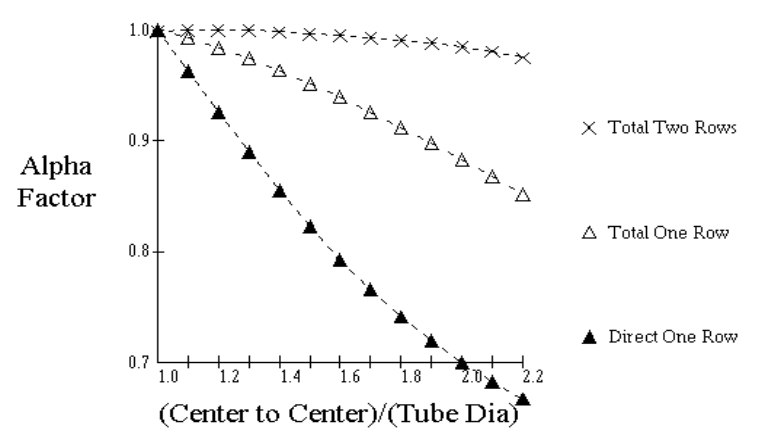
\includegraphics[scale=0.45]{images/alpha}
\caption[Efectividad de absorción para banco de tubos]{Efectividad de absorción para banco de tubos.} 
\label{fig:alpha}
\end{center}
\end{figure}
\par La curva correspondiente para una fila de tubos simple frente a la pared refractaria fue ajustada a una ecuación de 4to grado que representa la dependencia del factor alfa con la relación distancia de tubos con el diámetro del tubo ($Rel_{CC/D}$), se obtiene:
\begin{equation}
    \alpha = 1 + 0,49\frac{Rel_{cc/D}}{6} -0,09275(Rel_{cc/D})^2 +
     0,065\frac{(Rel_{cc/D})^3}{6} + 0,00025(Rel_{cc/D})^4
\end{equation}

\subsubsection{Factor global de transferencia radiante $(F)$}
\par Debido a que los gases de combustión en el horno no son un medio ideal de radiación, la ecuación \ref{eq:radiac} debe ser corregida usando un factor de transferencia radiante, dependiente de la emisividad del gas y la relación del área refractaria de plano frontal. Como el calor de radiación es reflejado de regreso a los tubos, por refracción, un horno con mayor relación de superficie refractaria con respecto a la superficie de los tubos, absorberá mas calor. Como los tubos no absorben perfectamente el calor, las curvas se basan en superficies de tubos con absorción de 0,9, un valor considerado como típico para superficies de metales oxidados. El factor de transferencia radiante final puede ser tomado de la siguiente curva (Figura \ref{fig:f}) ofrecida por Mekler \& Fairall \cite{bib:mekler}.
\begin{figure}[H]
\begin{center}
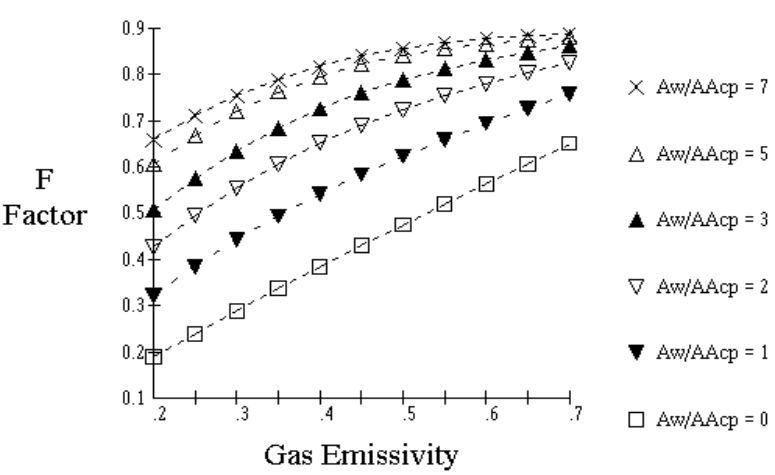
\includegraphics[scale=0.45]{images/f}
\caption[Factor de transferencia radiante, F]{Factor de transferencia radiante, F.\cite{bib:mekler}}
\label{fig:f}
\end{center}
\end{figure}

\par La relación, $Aw$/$\alpha Acp$, que aparece en el gráfico, es calculada con la ecuación \ref{eq:aw-acp}. El área de plano frontal efectiva, $\alpha Acp$, es el producto del factor de efectividad y del área de plano frontal como se describió anteriormente. Área refractaria efectiva se calcula con:
\begin{equation} \label{eq:aw}
Aw = Ar - \alpha Acp
\end{equation}
\par El área refractaria total, $Ar$, es el área de la sección de radiación, cubierta de material refractario, expuesta en la sección radiante del horno. Cuando hay sección de escudo, que recibe radiación directa, el $\alpha Acp$ para la sección radiante y para la sección de escudo se calculan de forma independiente y luego son sumados para calcular el factor de transferencia radiante.
\par La ecuación \ref{eq:aw} se puede reescribir como:
\begin{equation}
Aw = Ar - ((\alpha Acp)_{rad} + (\alpha Acp)_{esc})   
\end{equation}
\par Para finalmente obtener la siguiente ecuación:
\begin{equation} \label{eq:aw-acp}
Aw/\alpha Acp = \frac{Aw}{(\alpha Acp)_{rad} + (\alpha Acp)_{esc}}
\end{equation}

\par Para usar la gráfica de la Figura \ref{fig:f} en el simulador se creó la Tabla \ref{tbl:f-fac}, mostrada a continuación, y se realizó un doble ajuste para ser usada por el simulador.
\begin{table}[H]
\caption{Factor global de transferencia radiante con emisividad y $Aw/\alpha Acp$}
\label{tbl:f-fac}
\centering
\begin{tabular}{c|c|c|c|c|c|c}
\multirow{2}{5em}{Emisividad}&\multicolumn{6}{c}{$Aw/\alpha Acp$}\\
        & 0	    & 1	    & 2	    & 3 	& 5	    & 7     \\
\hline
0,20    & 0,189	& 0,323	& 0,427	& 0,506	& 0,607	& 0,658 \\
0,25    & 0,24	& 0,385	& 0,495	& 0,575	& 0,669	& 0,710 \\
0,30	& 0,289	& 0,442	& 0,555	& 0,634	& 0,720	& 0,753 \\
0,35	& 0,337	& 0,493	& 0,607	& 0,684	& 0,762	& 0,789 \\
0,40	& 0,384	& 0,540	& 0,652	& 0,725	& 0,795	& 0,818 \\
0,45	& 0,430	& 0,583	& 0,691	& 0,760	& 0,821	& 0,840 \\
0,50	& 0,475	& 0,623	& 0,724	& 0,788	& 0,841	& 0,857 \\
0,55	& 0,519	& 0,660	& 0,754	& 0,812	& 0,856	& 0,869 \\
0,60	& 0,563	& 0,694	& 0,780	& 0,831	& 0,867	& 0,878 \\
0,65	& 0,607	& 0,727	& 0,804	& 0,847	& 0,874	& 0,883 \\
0,70	& 0,651	& 0,758	& 0,825	& 0,862	& 0,880	& 0,886 \\
\end{tabular}
\end{table}

\par El primer ajuste, de la Tabla \ref{tbl:f-coef}, para obtener el factor global de transferencia radiante con la emisividad de los gases de combustión y $Aw/\alpha Acp$, usando la siguiente ecuación cuadrática:
\begin{equation}
\label{eq:f-fac}
F = A + B*emisividad + C*emisividad^2
\end{equation}
\begin{table}[H]
\caption{Coeficientes para el factor global de transferencia radiante dependientes del área refractaria efectiva $Aw/\alpha Acp$}
\label{tbl:f-coef}
\centering
\begin{tabular}{c|c|c|c}
$Aw/\alpha Acp$	&A	        & B	        &C      \\
\hline
0	    &-0,0157	& 1,0605	&-0,1571\\
1	    & 0,0592	& 1,4717	&-0,6825\\
2	    & 0,1320	& 1,7077	&-1,0354\\
3	    & 0,2047	& 1,7803	&-1,2149\\
5	    & 0,3356	& 1,6386	&-1,2429\\
7	    & 0,4227	& 1,4176	&-1,0890\\
\end{tabular}
\end{table}

\par El segundo ajuste, para interpolar en los valores de $Aw/\alpha Acp$ a los coeficientes de \ref{eq:f-fac}, se usó la siguiente ecuación cúbica, con los valores de la Tabla \ref{tbl:aw-fac}.
\begin{equation}
\label{eq:aw-fac}
A, B, C = -a(Aw/\alpha Acp)^3+b(Aw/\alpha Acp)^2+c(Aw/\alpha Acp)+d
\end{equation}
\begin{table}[H]
\caption{Subcoeficientes para el factor global de transferencia radiante}
\label{tbl:aw-fac}
\centering
\begin{tabular}{c|c|c|c|c}
    &	a	    & b         & c         &d      \\
    \hline
A	& -0,0005	& 0,0022	&0,0713	    &-0,0152\\
B	& 0,0072 	& -0,1195	&0,5333	    &1,0577 \\
C	& -0,0062   & 0,1168	&-0,6473	&-0,154 \\
\end{tabular}
\end{table}


\subsubsection{Emisividad de gases de combustión}
\par La emisividad de los gases de combustión se aproxima por las curvas presentadas por Lobo y Evans \cite{bib:rad}, correlacionada como una función de la suma de las presiones parciales del vapor de agua y el dióxido de carbono (P $= p_{H_2O} + p_{CO_2}$), multiplicada por la longitud media del haz radiante producida (L $= MBL$), (PL, Ec. \ref{eq:pl}), y dependiente de la temperatura de los gases de combustión, Tg. Variaciones en la temperatura de pared de los tubos entre 600°F y 1200°F causan una desviación menor a 1\% de estas curvas.
\begin{figure}[H]
\begin{center}
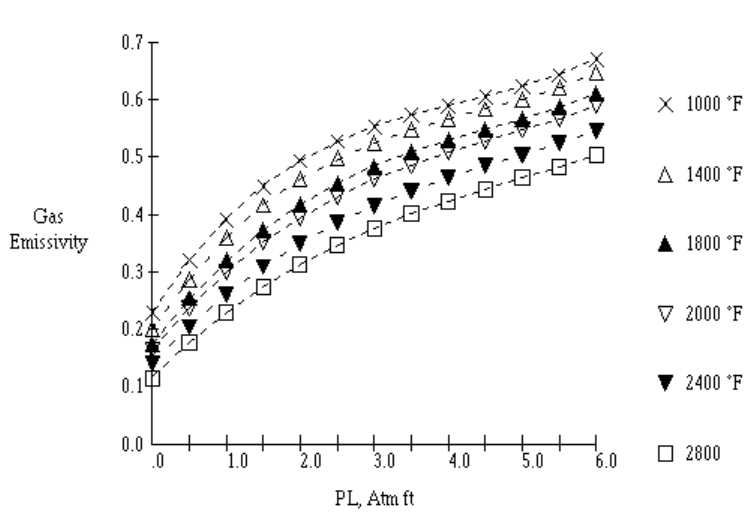
\includegraphics[scale=0.42]{images/emiss}
\caption[Emisividad de gases de combustión]{Emisividad de gases de combustión.\cite{bib:mekler}}
\label{fig:emiss}
\end{center}
\end{figure}
\begin{equation}
\label{eq:pl}
PL = (PH_2O + PCO_2) * MBL
\end{equation}
\par Donde $PH_2O$ y $PCO_2$ son las presiones parciales del agua y dióxido de carbono en el gas, y MBL en pies obtenido de la tabla \ref{tbl:mbl}.
\par A partir de la la Figura \ref{fig:emiss} se creó la Tabla \ref{tbl:pl}, con los valores extraídos de las curvas, y con la finalidad de obtener las funciones necesarias para calcular la emisividad en el simulador.
\begin{table}[H]
\caption{Emisividad de los gases de combustión a partir de PL y temperatura}
\label{tbl:pl}
\centering
\begin{tabular}{c|c|c|c|c}
PL	& 1.000 $^o$F   & 1.400 $^o$F   & 1.800 $^o$F   & 2.000 $^o$F\\
\hline
0,1	& 0,143	        & 0,118	        & 0,102	        & 0,095\\
0,5	& 0,230	        & 0,201	        & 0,175	        & 0,163\\
1,0	& 0,320	        & 0,288	        & 0,254	        & 0,237\\
1,5	& 0,392	        & 0,359	        & 0,320         & 0,299\\
2,0	& 0,450	        & 0,416	        & 0,374	        & 0,352\\
3,0	& 0,528	        & 0,497	        & 0,454	        & 0,431\\
4,0	& 0,574	        & 0,548	        & 0,508	        & 0,486\\
5,0	& 0,606	        & 0,584	        & 0,548	        & 0,528\\
6,0	& 0,644	        & 0,622	        & 0,587	        & 0,567\\
\end{tabular}
\end{table}
\par El primer ajuste para encontrar la emisividad, dependiente de PL para cada temperatura de los gases en la sección de radiación, con los coeficientes resultantes en la Tabla \ref{tbl:emisividad}, desarrollado de la siguiente ecuación cúbica:
\begin{equation}
\label{eq:emisividad}
E = A + B*PL + C*PL^2 + D*\frac{PL^3}{10}
\end{equation}
\begin{table}[H]
\caption{Coeficientes para calcular la emisividad de los gases de combustión a partir de PL y temperatura}
\label{tbl:emisividad}
\centering
\begin{tabular}{c|c|c|c|c}		
Temp.	    & A	        & B	        & C 	    & D     \\
\hline
1.000 $^o$F	& 0,1194	& 0,2421	& -0,0448	& 0,0032\\
1.400 $^o$F	& 0,0957	& 0,2293	& -0,0400	& 0,0027\\
1.800 $^o$F	& 0,0819	& 0,2027	& -0,0326	& 0,0021\\
2.000 $^o$F	& 0,0764	& 0,1871	& -0,0284	& 0,0018\\
\end{tabular}
\end{table}

\par El segundo ajuste, se crea para interpolar los valores de los coeficientes usados en la Ecuación \ref{eq:emisividad}, en función de la temperatura (Ec. \ref{eq:emisividad-fac}); ajuste con los coeficientes mostrados en la Tabla \ref{tbl:emisividad-fac}.
\begin{equation}
\label{eq:emisividad-fac}
A, B, C, D = a*T^2+b*T+c
\end{equation}
\begin{table}[H]
\caption{Subcoeficientes para calcular la emisividad de los gases de combustión en función de la temperatura}
\label{tbl:emisividad-fac}
\centering
\begin{tabular}{c|c|c|c}		
	& a         & b	        & c \\
	\hline
A	&  2,58E-08	& -1,19E-04	& 0,212580 \\
B	& -3,90E-08	&  5,60E-05	& 0,225800 \\
C	&  6,80E-09	& -4,10E-06	&-0,047351 \\
D	& -2,20E-10	& -7,20E-07	& 0,004165 \\
\end{tabular}
\end{table}

\subsubsection{\ac{mbl}}
\par La longitud media del haz radiante es definida como la distancia de la llama al banco de tubos en la sección de radiación, por lo cual la distribución de los tubos debe ser tomada en cuenta. Si el horno es de base rectangular con tubos en el centro, \ac{mbl} será la mitad del área rectangular del horno. Para otras configuraciones, como un horno cilíndrico con una disposición de tubos octagonal o tubos cruzados, \ac{mbl} deberá ser calculada con esas consideraciones.
\par \ac{mbl} para hornos puede ser tomada, de acuerdo a Wimpress \cite{bib:wimpress}, como se muestra en la Tabla \ref{tbl:mbl}.
\begin{table}[H]
\caption[Cálculo de MBL]{Cálculo de MBL con dependencia de las dimensiones de la sección de radiación}
\label{tbl:mbl}
\centering
\begin{tabular}{c|c}
    Relación de dimensión de la cámara  & Longitud media del haz radiante \\
    \hline
    1-1-1 a 1-1-3   & \multirow{2}{12em}{$\frac{2}{3}$ (Vol. Cámara Comb.)$^{1/3}$} \\
    1-2-1 a 1-2-4   & \\
    \hline
    1-1-4 a 1-1-inf & 1 * Menor dimensión \\
    \hline
    1-2-5 a 1-2-inf   & 1,3 * Menor dimensión \\
    \hline
    1-3-3 a 1-inf-inf & 1,8 * Menor dimensión \\
    \hline
    \multicolumn{2}{c}{Para hornos cilíndricos verticales} \\
    \hline
    Largo/Diámetro $<$ 2  & (($\frac{L}{D}$-1)*0,33 + 0,67)*D\\
    \hline
    Largo/Diámetro $\geq$ 2 & Diámetro\\
\end{tabular}
\end{table}

\subsection{Zona Escudo}
\par “Esta zona está conformada por dos o tres hileras de tubos lisos ubicadas en la parte inferior de la sección de convección. Actúa como un escudo de protección de los tubos convectivos provistos de superficies extendidas (pernos, aletas, etc.) y reciben aproximadamente la misma cantidad de calor tanto por radiación como por convección.
\par Realizando un balance de energía en la zona de los tubos de escudo se obtiene:
\begin{equation}
\label{eq:esc}
Q_{ESC} = Q_{ge} + Q_{radEsc} = \dot m_{f} *C_{p_f} *(T_{fer} - T_{fee})
\end{equation}
\par Donde $Q_{radEsc}$ es el calor por radiación que proviene directamente de la zona radiante hacia el escudo de tubos y que fue calculado al determinar la temperatura efectiva de radiación $T_g$. La temperatura de entrada del gas a la zona de escudo $T_{gr}$ es igual a la temperatura efectiva $T_g$, lo cual se infiere de haber supuesto una temperatura de mezcla ideal de los gases en la sección radiante. $T_{gr} = T_g$
\par Rearreglando la ecuación \ref{eq:esc} se obtiene:
\begin{equation}
Q_{fs} - Q_{fe} = Q_{gr} - Q_{ge} + Q_{radEsc}
\end{equation}
\par Donde,
\begin{equation}
\label{eq:qesc}
\dot m_{f} *C_{p_f} *(T_{fer} - T_{fee}) = 
\dot m_{g} *C_{p_g} *(T_{gr}  - T_{ge}) + Q_{radEsc}
\end{equation}
\begin{equation} \label{eq:esc-radi}
Q_{radEsc} = \sigma *(\alpha *Acp )_{ESC} *F *(T_{gr}^4 -T_w^4)
\end{equation}
\par Para los gases de combustión, el cambio de energía dentro de la zona escudo se debe a la transferencia de calor hacia los tubos.
\begin{equation}
\label{eq:qesc-lmtd}
\dot m_{g} *C_{p_g} *(T_{gr} -T_{ge}) = U_0 *A_0 *LMTD
\end{equation}
\par Donde LMTD es la Diferencia de Temperatura Media Logarítmica entre los gases de combustión y el fluido del proceso, expresada por:
\begin{equation}
\label{eq:lmtd}
   LMTD = \frac{(T_{gr}-T_{fer}) - (T_{ge}-T_{fee})}
   {ln[(T_{gr}-T_{fer}) /(T_{ge}-T_{fee})]}
\end{equation}
Sustituyendo (\ref{eq:qesc-lmtd}) en (\ref{eq:qesc})
\begin{equation}
\label{eq:tesc}
  Q_{ESC} = \dot m_{f} *C_{p_f} *(T_{fer} - T_{fee}) = U_0 *A_0 *LMTD + Q_{radEsc}
\end{equation}

\subsubsection{Coeficiente global de transferencia de calor en la zona escudo}
\par Generalmente el escudo de tubos está formado por dos o tres filas de tubos lisos (sin aletas) pero formando parte del banco de tubos de la sección superior del horno que incluye otra zona de tubos con aletas, para un banco de tubos lisos el coeficiente global de transferencia de calor viene dado por la ecuación:
\begin{gather*}
\label{}
U_0  = 1 / \Sigma R \\
\Sigma R = R_{ext} + R_{tubo} + R_{int}
\end{gather*}
\par Donde $R_{ext}, R_{tubo}, R_{int}$ son la resistencia externa de la pared del tubo, la resistencia interna del tubo y el factor de ensuciamiento interno respectivamente.
\par Sustituyendo:
\begin{equation}
\label{}
\Sigma R = \frac{1}{h_o} +\frac{d_o*ln(d_o/d_i)}{2*k_t} +\frac{A_o}{A_i*h_i} +R_{fi}
\end{equation}
\begin{equation}
\label{}
\dot m_{g} *C_{p_g} *(T_{gr} - T_{ge}) = \frac{A_0 *LMTD}
{\frac{1}{h_o} +\frac{d_o*ln(d_o/d_i)}{2*k_t} +\frac{d_o}{d_i*h_i} +\frac{d_o}{d_i}R_{fi}}
\end{equation}
\par Donde el coeficiente interno de película se calcula como en el caso de los tubos de la sección radiante mediante la ecuación \ref{eq:hi}:
\par El coeficiente externo $h_o$ puede ser expresado como la sumatoria de las resistencias externas como:
\begin{equation}
\label{eq:ho}
h_o = 1/(\frac{1}{h_c + h_{r}} + R_{fe})
\end{equation}
\par Donde \\
$h_c$ es el coeficiente de película externo de transferencia de calor.\\
$h_r$ es el coeficiente efectivo de radiación hacia la pared del tubo.\\
$R_{fe}$ es el factor de ensuciamiento externo.\\
\par El coeficiente de película exterior para un banco de tubos lisos colocados triangularmente (tresbolillo) puede ser calculado por:
\begin{equation}
\label{eq:hc}
\begin{gathered}
h_c = 0,33 * \frac{k_g}{d_o} *Pr^{1/3} *Re^{0,6} |_g\\
h_c = 0,33 * \frac{k_g}{d_o} *Pr^{1/3}|_g*(\frac{d_o*G_n}{\mu_g})^{0,6}
\end{gathered}
\end{equation}
$G_n$ es la velocidad másica basada en el área libre para el flujo de los gases, es decir, el espacio entre los tubos por el largo del horno.
\par El coeficiente efectivo de radiación, que se aplica al calor por radiación que transfieren los gases de combustión, sumado al calor reradiado de las paredes de la zona de escudo, a la pared de los tubos, es aproximado con la siguiente ecuación empírica:
\begin{equation}
\label{eq:hr}
h_r = 0,092*T_g - 34  
\end{equation}
\par Donde $T_g$ es la temperatura de los gases en K y $h_r$ viene expresado en kJ/m$^2$h°C

\subsubsection{Factor de efectividad del banco de tubos de la zona escudo $(\alpha)_{ESC}$}
\par Dado que todo el calor por radiación hacia este banco de tubos sale de la sección radiante y es absorbido por los tubos, el factor de efectividad de absorción, $\alpha$, para los tubos de la zona escudo (Ec. \ref{eq:esc-radi}) puede tomarse como igual a uno.

\subsubsection{Área de plano frontal que reemplaza el área de los tubos $(Acp)_{ESC}$}
\par El área de plano frontal para la zona de escudo es igual al área de plano frontal definida en la zona radiante para la primera fila de tubos de esta sección.
\begin{equation}
Acp = \frac{N_{tubo}}{2} * S_{tubo} * {L_tubo}
\end{equation}
\par Donde, \\
$N_{tubo}$ = Número de tubos. \\
$S_{tubo}$ = Espaciado de tubos. \\
$L_{tubo}$ = Largo efectivo del tubo.

\par Los valores usados para el factor global de transferencia radiante, F, temperatura efectiva del gas en la cámara de radiación, $T_{gr}$, y temperatura promedio de pared de tubos, $T_w$, son los mismos valores usados en la sección radiante.

\subsubsection{Temperatura máxima en los tubos de la zona escudo}
\par Según han reportado Mekler \& Fairall la radiación luminosa desde la sección radiante a los tubos de la zona escudo, $Q_{radEsc}$ puede ser repartida 76,92\% en la primera fila y 23,08\% restante en la segunda fila \cite{bib:mekler}. Esta aproximación conjuntamente con la distribución del flujo de calor es usada para calcular la temperatura máxima de pared en los tubos de la zona de escudo.
\par Similarmente, se puede considerar que el flujo de calor convectivo en la primera fila ocurre entre el gas a la temperatura de entrada $T_{gr}$ y el fluido a la temperatura de salida $T_{fer}$, así:
\begin{equation}
Q_{ESC}|_{1^{\circ} fila} = A_0|_{1^{\circ} fila}*U_0*(T_{gr} - T_{fer}) + 0,7692 Q_{radEsc}
\end{equation}
\par Dividiendo por $A_0|_{1^{\circ} fila}$:
\begin{equation}
q\prime_{ESC}|_{1^{\circ} fila} = U_0*(T_{gr} - T_{fer}) + 0,7692 q\prime_{radEsc}
\end{equation}
\par Finalmente, la temperatura de pared del tubo en la primera fila:
\begin{equation}
T_w|_{1^{\circ} fila} = T_{fer} + q\prime_{ESC}|_{1^{\circ} fila} *[(d_0/d_i ) [R_{fi} + 1/h_i + d_i*Ln(d_0/d_i)/(2k_w)]
\end{equation}
\par Este análisis supone una temperatura uniforme circularmente. $U_0$, $T_{fer}$, $T_{gr}$ previamente calculados al cerrar el balance de energía en la simulación del horno.

\subsection{Zona Convectiva}
\par En esta zona el calor del gas hacia los tubos se transfiere en forma similar al de la zona escudo. En el lado exterior de los tubos se trasfiere calor por radiación y por convección en paralelo, pero en este caso la presencia de las aletas modifica el cálculo de los coeficientes de transferencia de calor.
\par El balance de energía en esta zona depende únicamente de la energía entrando y saliendo de los gases de combustión y del fluido del proceso, resultando en:
\begin{equation}
\label{eq:conv}
Q_{CONV} = Q_{g_c} = \dot m_{f} *C_{p_f} *(T_{f_e} - T_{f_{ee}})
\end{equation}
\par Rearreglando:
\begin{equation}
Q_{f_{ee}} - Q_{f_e} = Q_{g_e} - Q_{g_s}
\end{equation} \begin{equation} \label{eq:qconv}
\dot m_{f} *C_{p_f} *(T_{f_e} - T_{f_{ee}}) = 
\dot m_{g} *C_{p_g} *(T_{ge}  - T_{gs}) = Q_{CONV}
\end{equation}
\par Los valores de $C_{p_f}$ y $C_{p_g}$ son calculados a la temperatura promedio del fluido y del gas.

\subsubsection{Transferencia convectiva, tubos con aletas}
\par Las ecuaciones de transferencia de calor para los tubos con aletas son básicamente las mismas que para los tubos lisos exceptuando al coeficiente externo, $h_c$, donde se introduce un nuevo concepto para explicar la aleta o superficie extendida.

\subsubsection{Coeficiente global de transferencia de calor, $U_0$}
\par El calor proveniente de los gases de combustión que se transfiere al fluido en la sección de convección esta definido por la ecuación:
\begin{equation}
\dot m_{g} *C_{p_g} *(T_{ge}  - T_{gs}) = U_0 *A_0 *LMTD
\end{equation}
\par Donde $U_0$ definido como el inverso de la suma de las resistencias de transferencia de calor:
\begin{gather}
\label{}
U_0  = 1 / \Sigma R \\
\Sigma R = R_{ext} + R_{tubo} + R_{int} \\
\Sigma R =  \frac{1}{h_{c}} 
            +\frac{d_o*ln(d_o/d_i)}{2*k_t} 
            +(\frac{1}{h_i}+R_{fi})*\frac{d_o}{d_i} 
\end{gather}

\subsubsection{Coeficiente externo de transferencia de calor, $h_{c}$}
\par El coeficiente externo de transferencia de calor es calculado tomando en consideración la presencia de aletas en los tubos.
\begin{equation}
h_{c} = h_o * (E *Af_0 +Ap_0) / A_0
\end{equation}

\par Donde,\\
$E$ = Eficiencia de las aletas.\\
$A_0$ = Área de superficie externa total.\\
$Af_0$ = Área de superficie externa de aletas. \\
$Ap_0$ = Área de superficie lisa de tubos.
\par Y, $h_o$, coeficiente externo promedio de transferencia de calor: 
\begin{equation}
h_o = 1/(\frac{1}{h_e+h_r}+R_{fe})
\end{equation}

\par Donde,\\
$h_r$ = Coeficiente externo de radiación de transferencia de calor.\\
$R_{fe}$ = Resistencia de ensuciamiento externo.
\par Y, $h_e$, coeficiente de película efectivo externo de transferencia de calor: 
\begin{equation}
h_e = j *G_n *C_{p_g} *Pr^{0,67}|_g
\end{equation}

\par Donde,\\
$j$ = Factor Colburn de transferencia de calor.\\
$G_n$ = Velocidad másica basada en el área libre neta.\\
$Pr$ = Número de Prandtl $(\mu*C_p /k)_{gb}$ evaluado a $T_{gb}$.\\
$C_{p_g}$ = Capacidad calorífica del gas.\\
$k_g$ = Conductividad térmica del gas.\\
$\mu_g$ = Viscosidad dinámica del gas.

\subsubsection{Factor Colburn de transferencia de calor, j}
\par Dado por la siguiente correlación \cite{bib:colburn}.
\begin{equation}
j = C_1 *C_3 *C_5 *(\dfrac{d_f}{d_o})^{0,5} *(\frac{T_b}{T_s})^{0,25}
\end{equation}
\par Donde, \\
$C_1$ = Corrección del número de Reynolds. \\
$C_3$ = Corrección geométrica. \\
$C_5$ = Corrección no-equilateral y de fila. \\
$d_f$ = Diámetro externo de la aleta. \\
$d_o$ = Diámetro externo del tubo. \\
$T_b$ = Temperatura promedio del gas, K. \\
$T_s$ = Temperatura promedio de aleta, K.
\par Corrección del número de Reynolds:
\begin{equation}
C_1 = 0,25 *Re^{-0,35}
\end{equation}
\par Corrección geométrica (para aletas sólidas en patrón escalonado):
\begin{equation}
C_3 = 0,35 +0,65 *e^{-0,25*l_f/s_f}
\end{equation}
\par Donde, \\
$l_f$ = Altura de aleta. \\
$s_f$ = Espaciado de aleta.
\par Corrección no-equilateral y de fila (para tubos aletados en patrón escalonado):
\begin{equation}
C_5 = 0,7 +(0,70 -0,8 *e^{-0,15 *N_r^2}) *e^{-P_l/P_t}
\end{equation}
\par Donde, \\
$N_r$ = Numero de tubos por fila. \\
$P_l$ = Paso de tubo longitudinal.\\
$P_t$ = Paso de tubo transversal. \\

\subsubsection{Cálculo de la temperatura máxima en la aleta}
\par La distribución de temperatura en aletas es un problema clásico en la
literatura de transferencia de calor por conducción, incluyendo aletas de área conductiva variable como son las aletas trapezoidales y las aletas anulares. En estas últimas la solución de la ecuación diferencial resulta en funciones de Bessel de primer y segundo orden que en la práctica son complicadas de evaluar.
\par Una simplificación del problema es la de utilizar la solución para aletas de área constante y despreciar el calor por convección en la punta de le aleta, lo cual resulta en la siguiente distribución de temperatura:
\begin{equation}
(T_x -T_g )/(T_w - T_g) = \frac{cosh(m(L-x))}{cosh(mL)}
\end{equation}
\par Donde $m = (h_0 / \delta k)$ y $\delta = x/2$
\par Evaluando para x=L resulta en
\begin{equation}
(T_p - T_g )/(T_w -T_g ) = 1 / cosh(mL)
\end{equation}
\par Aplicando la ecuación al caso de la sección convectiva del horno para la primera fila \\
$T_p = T_ge + (T_w -T_{ge}) / cosh(mL)$
\par La temperatura de pared del tubo debe ser estimada para la primera fila $Q_{CONV}|_{1^{\circ} fila} = A_0|_{1^{\circ} fila} *U_0 *
(T_{ge} - T_{fee})$
\par Y el flujo de calor por unidad de área $q\prime_{CONV}|_{1^{\circ} fila} = U_0 * (T_{ge} - T_{fee})$
\begin{equation}
T_w|_{1^{\circ} fila} = T_{fee} + q\prime_{conv}|_{1^{\circ} fila} *
[(d_0 /d_i ) [ R_{fi} + 1/h_i + d_i*Ln(d_0 /d_i)/(2k_f)]
\end{equation}

\subsubsection{Coeficiente de radiación del gas, $h_r$}
\par Puede ser aproximado con las correlaciones usadas por Lobo \& Evans \cite{bib:rad}. Este coeficiente se utiliza para calcular el coeficiente global de transferencia de calor para tubos lisos y tubos con aletas. 
Para tubos lisos,
\begin{equation}
h_r = 2,2 *\gamma_r *PL^{0,50}
\end{equation}

\par Y para tubos con aletas,
\begin{equation}
h_r = 2,2 *\gamma_r *PL^{0,50} *(Ap_0/A_0) *0,75
\end{equation}

\par Donde,\\
PL tomado de la ecuación \ref{eq:pl}.\\
$\gamma_r$ = Factor de radiación externo.\\
$Ap_0$ = Área de superficie expuesta de tubos lisos.\\
$A_0$ = Área de superficie externa total. \\
\par El factor de radiación externo puede ser hallado en las curvas experimentales de Lobo \& Evans de la Figura \ref{fig:gamma} y para este modelo se aproximó a 2,2 * (3,6 kJ/m²h°C).
\begin{figure}[H]
\begin{center}
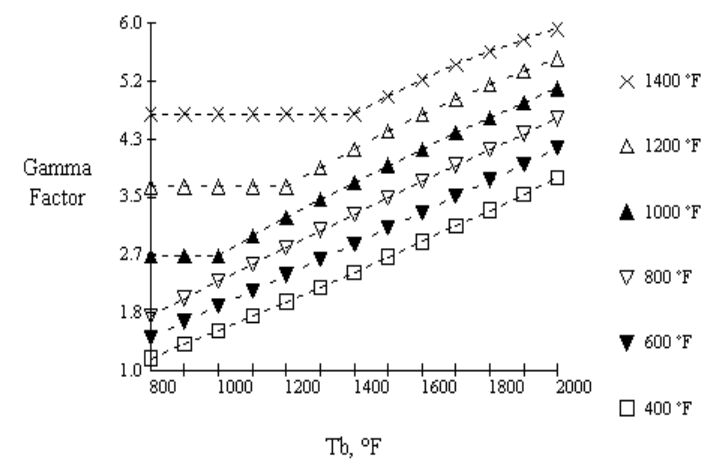
\includegraphics[scale=0.40]{images/gamma}
\caption[Factor de radiación externo]{Factor de radiación externo. Este gráfico requiere de la temperatura promedio del gas y de la temperatura promedio de la superficie del tubo.\cite{bib:rad}}
\label{fig:gamma}
\end{center}
\end{figure}

\subsubsection{Eficiencia térmica en hornos}
\par El cálculo de eficiencia tomado del estándar API 560 \cite{bib:api560} se reduce a calcular la relación entre el calor suministrado sin contar las pérdidas de calor y el calor cedido en la combustión.
\begin{equation}
Eficiencia = 100 *\frac{\dot m_c*NCV +Q_a +Q_c -Q_{perdidas} -Q_{chimenea}
}{\dot m_c*CV +Q_a +Q_c}
\end{equation}
\par Y, a su vez, el calor de combustión puede ser calculado a partir del poder calorífico inferior (NCV) o el poder calorífico superior (GCV), obteniendo dos posibles valores:
\begin{gather}
Eficiencia_{[@NCV]} = 100 *\frac{\dot m_c*NCV +Q_a +Q_c -Q_{perdidas}-Q_{chimenea}
}{\dot m_c*NCV +Q_a +Q_c}\\
Eficiencia_{[@GCV]} = 100 *\frac{\dot m_c*NCV +Q_a +Q_c -Q_{perdidas} -Q_{chimenea}
}{\dot m_c*GCV +Q_a +Q_c}
\end{gather}